\documentclass[../main]{subfiles}

\begin{document}

\section{Functions and Linear Graphs}

\subsection{Cartesian Coordinates}

The \textbf{Cartesian coordinate system} describes the positions of points and
lines in a plane. A Cartesian plane consists of a horizontal axis and a vertical
axis.
\begin{enumerate}
\item The horizontal axis: \textbf{x-axis}
\item  The vertical axis: \textbf{y-axis}
\item The two axes intersect at the origin, \(O\).

\end{enumerate}

The position of any point on the Cartesian plane is represented as an ordered
pair \((a,b)\) of real numbers know as \textbf{coordinates}.

Note:
\(a\) is know as the \(x-coordinate\)

\(b\) is know as the \(y-coordinate\)

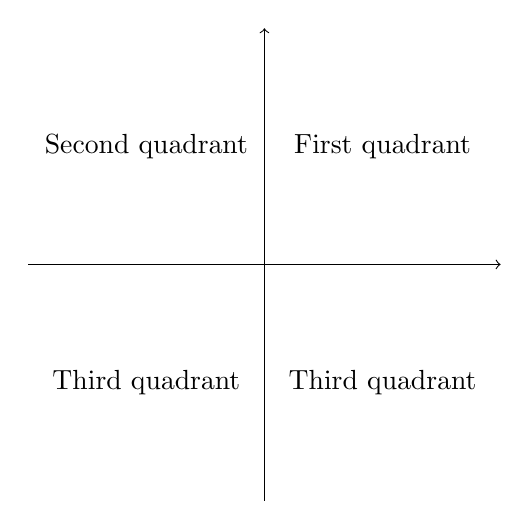
\begin{tikzpicture}[scale=1.5]
  \coordinate (0) at (0,0);
  \draw [->] (-2, 0 ) -- (2,0);
  \draw [<-] (0,2) -- (0,-2) ;
  \node at (1,1) []{First quadrant};
  \node at (-1,1) []{Second quadrant};
  \node at (-1,-1) []{Third quadrant};
  \node at (1,-1) []{Third quadrant};

\end{tikzpicture}

The position of any point on the Cartesian plane is represented as an ordered
pair(a,b) of real numbers known as \textbf{coordinates}.

\begin{tikzpicture}
  \draw [->]  (-2,0) -- (2, 0) ;
  \draw [<-] (0,2) -- (0, -2);
  \draw [densely dotted] (1, 0) -- (1,1) -- (0, 1);
  \node at (1,0)[below] {$a$};
  \node at (0,1)[left] {$b$};
  \node at (2,0) [right] {$x$};
  \node at (0,2)[above] {$y$};
  \node at (0,0)[left,below] {$O$};
  \node at (1,1)[circle,fill=black]{};
\end{tikzpicture}

Notes:
\begin{itemize}
\item \(a\) is known as the \(x-\)coordinate.
\item \(b\) is known as the \(y-\)coordinate.
\item the coordinate of the origin is \((0,0)\).
\end{itemize}

\begin{tikzpicture}

\begin{axis}[xshift=9cm,
    xmin=-11,xmax=11,
    ymin=-11,ymax=11,
    grid=both,
    axis lines=middle,
    minor tick num=5,
    enlargelimits={abs=0.5},
    axis line style={latex-latex},
    ticklabel style={font=\tiny,fill=white},
    xlabel style={at={(ticklabel* cs:1)},anchor=north west},
    ylabel style={at={(ticklabel* cs:1)},anchor=south west}
]

\coordinate (O) at (0,0);
\node[fill=white,circle,inner sep=0pt] (O-label) at ($(O)+(-135:10pt)$) {$O$};

\end{axis}
\end{tikzpicture}
\end{document}